\section{¿Qué es el NLP?}\label{que-es-la-nlp}
El \textbf{procesamiento de lenguaje natural} (NLP, por sus siglas en inglés) es una tecnología de \textbf{machine learning} que permite a las computadoras interpretar, manipular y comprender el lenguaje humano. Gracias al NLP, las máquinas pueden interactuar con las personas utilizando lenguaje cotidiano de manera eficaz. Esto incluye tareas como el análisis de texto, la traducción automática, y la generación de respuestas a preguntas en lenguaje natural.

\begin{tikzpicture}[node distance=2cm]
    % Input (Entrada) con color
    \node (input) [draw, rectangle, fill=cyan!30, text width=6cm, align=left, rounded corners] 
    {Texto en lenguaje natural \\ \textbf{Ejemplo:} ``¿Cuántas unidades se produjeron hoy?''};
    
    % Procesamiento NLP con color
    \node (process) [below=of input, draw, rectangle, fill=yellow!30, text width=6cm, align=left, rounded corners] 
    {Procesamiento NLP \\ \textbf{Descripción:} El sistema descompone la frase, identifica palabras clave como ``unidades'' y ``hoy'', y analiza el contexto.};
    
    % Output (Salida) con color
    \node (output) [below=of process, draw, rectangle, fill=green!30, text width=6cm, align=left, rounded corners] 
    {Respuesta generada \\ \textbf{Ejemplo:} ``Se produjeron 500 unidades''};
    
    % Flechas de conexión con color
    \draw[->, thick, blue] (input) -- (process);
    \draw[->, thick, blue] (process) -- (output);
    
    % Descripción adicional debajo del diagrama
    \node at (-3, -11) [text width=15cm, align=center] 
    {Este diagrama muestra cómo funciona el procesamiento de lenguaje natural (NLP): el usuario introduce una pregunta en lenguaje natural (entrada), el sistema NLP la procesa, descomponiendo la frase e identificando el contexto, y luego genera una respuesta adecuada (salida).};
\end{tikzpicture}

\section{API: Interfaz de Programación de Aplicaciones}\label{api}
Una API (Interfaz de Programación de Aplicaciones) es un conjunto de reglas y especificaciones que facilita la comunicación e intercambio de datos entre distintas aplicaciones de software. Las APIs actúan como puentes digitales, permitiendo que diferentes tecnologías trabajen juntas sin problemas. Esto es esencial en un entorno moderno donde las aplicaciones y sistemas deben integrarse para ofrecer soluciones completas.

\subsection{Ventajas de las APIs}
Las APIs han revolucionado la forma en que las aplicaciones de software interactúan entre sí. Algunas de sus principales ventajas son:

\begin{itemize}
    \item \textbf{Reducción de costos y complejidad:} Permiten integrar servicios externos en lugar de desarrollar todo desde cero, lo que reduce tiempo, esfuerzo y costos de desarrollo.
    \item \textbf{Impulso a la innovación:} Los desarrolladores pueden aprovechar APIs existentes para acelerar el desarrollo de nuevas soluciones, lo que fomenta la creación rápida de productos innovadores.
    \item \textbf{Mejora de la experiencia de usuario:} APIs bien integradas permiten experiencias más completas y personalizadas al conectar diversas aplicaciones.
\end{itemize}

\subsection{Ejemplo Práctico}
Supongamos que estás desarrollando una aplicación financiera. En lugar de construir un sistema desde cero para manejar transacciones de criptomonedas, puedes utilizar la API de un servicio como \textbf{Gemini}. A través de esta API puedes realizar varias acciones, tales como:

\begin{itemize}
    \item Consultar precios de criptomonedas en tiempo real.
    \item Ejecutar órdenes de compra y venta.
    \item Realizar análisis de mercado en base a los datos obtenidos.
\end{itemize}

\section{La Nueva Era de la IA Generativa}\label{la-nueva-era-ia-generativa}

\subsection{Introducción a la Inteligencia Artificial en la Maquiladora}
En el mundo de las maquiladoras, la \textbf{inteligencia artificial (IA)} está teniendo un impacto significativo. Herramientas como \textbf{ChatGPT}, basadas en \textbf{procesamiento de lenguaje natural (NLP)}, permiten que la IA entienda y genere lenguaje humano, facilitando la interacción entre las máquinas y las personas sin la necesidad de interfaces complejas.

\subsection{Natural Language Processing (NLP): ¿Qué es y por qué es importante?}
El \textbf{procesamiento de lenguaje natural} permite a las máquinas comprender, procesar y generar lenguaje humano. Antes del NLP, las interacciones con las computadoras se limitaban a comandos técnicos y interfaces especializadas. Con el NLP, es posible interactuar con las máquinas utilizando el lenguaje cotidiano, lo que simplifica y democratiza el uso de la tecnología.

\subsection{Impacto del NLP en la Maquiladora}
El NLP tiene un impacto significativo en las maquiladoras, ya que permite una interacción más eficiente entre los trabajadores y las máquinas. Por ejemplo, un gerente podría preguntar en lenguaje natural: \textit{"¿Cuántas piezas defectuosas se produjeron hoy?"}, y recibir una respuesta rápida y detallada sin tener que navegar por complejas bases de datos.

\subsection{De las Interfaces Especializadas a la IA Conversacional}
Antes de herramientas como \textbf{ChatGPT}, las empresas dependían de interfaces complicadas para utilizar la IA. Hoy en día, la \textbf{IA conversacional} ha democratizado el acceso a esta tecnología, permitiendo que cualquier persona pueda interactuar con sistemas inteligentes a través de conversaciones naturales.

\section{Costos en Modelos de Lenguaje Extensos (LLMs)}\label{costo-en-llms}

\subsection{¿Qué es un Token?}\label{que-es-un-token}
En el contexto de los \textbf{modelos de lenguaje extensos (LLMs)}, como \textbf{GPT} o \textbf{Gemini}, un \textbf{token} es una unidad de información que representa una palabra, parte de una palabra, o incluso un símbolo de puntuación. Los LLMs procesan y generan texto basándose en estos tokens.

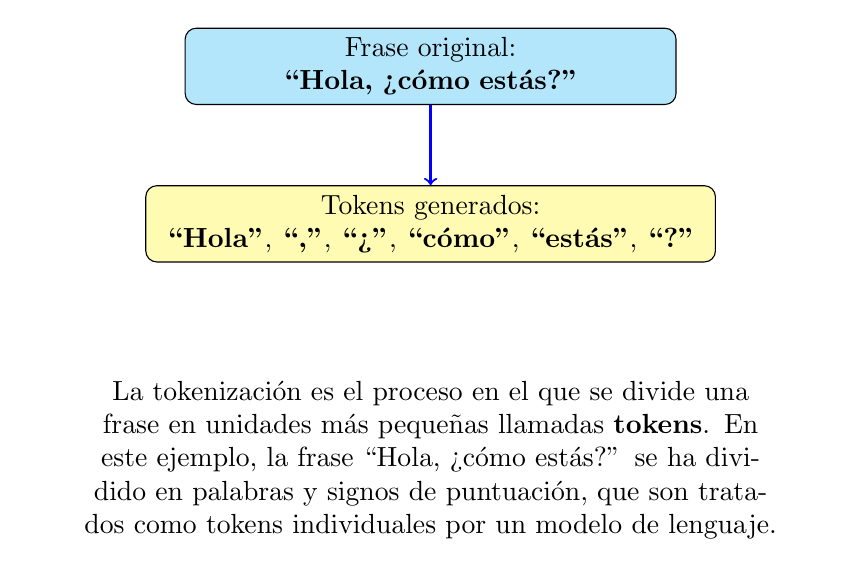
\begin{tikzpicture}[node distance=2cm]

    % Nodo para la frase original
    \node (phrase) [draw, rectangle, fill=cyan!30, text width=6cm, align=center, rounded corners] 
    {Frase original: \\ \textbf{``Hola, ¿cómo estás?''}};
    
    % Nodo para los tokens generados
    \node (tokens) [below of=phrase, draw, rectangle, fill=yellow!30, text width=7cm, align=center, rounded corners] 
    {Tokens generados: \\ \textbf{``Hola''}, \textbf{``,''}, \textbf{``¿''}, \textbf{``cómo''}, \textbf{``estás''}, \textbf{``?''}};
    
    % Conectar nodos con una flecha
    \draw[->, thick, blue] (phrase) -- (tokens);
    
    % Añadir un nodo de explicación
    \node (explanation) [below of=tokens, node distance=3cm, text width=10cm, align=center] 
    {La tokenización es el proceso en el que se divide una frase en unidades más pequeñas llamadas \textbf{tokens}. 
    En este ejemplo, la frase ``Hola, ¿cómo estás?'' se ha dividido en palabras y signos de puntuación, 
    que son tratados como tokens individuales por un modelo de lenguaje.};

\end{tikzpicture}

\subsection{El Cobro por Token}\label{el-cobro-por-token}
Los proveedores de IA, como OpenAI, cobran según la cantidad de tokens utilizados en una interacción. Esto incluye tanto los \textbf{tokens de entrada} (el texto que se envía al modelo) como los \textbf{tokens de salida} (la respuesta generada por el modelo). Este método de cobro es escalable y flexible, lo que lo hace adecuado para empresas de distintos tamaños.

\subsection{Ventajas del Cobro por Tokens}\label{ventajas-del-cobro-por-tokens}
\begin{itemize}
    \item \textbf{Escalabilidad:} Las empresas pueden empezar con un uso pequeño y aumentar conforme lo necesiten.
    \item \textbf{Eficiencia:} Se paga únicamente por el procesamiento real de los datos.
    \item \textbf{Previsión de costos:} Los costos son predecibles, ya que dependen del número de tokens generados en cada interacción.
\end{itemize}

\subsection{Retos del Cobro por Tokens}\label{retos-del-cobro-por-tokens}
Aunque el cobro por tokens es eficiente, también presenta algunos desafíos:
\begin{itemize}
    \item \textbf{Costos acumulativos:} En aplicaciones que requieren grandes volúmenes de datos o respuestas extensas, el costo puede aumentar rápidamente.
    \item \textbf{Dificultad para estimar los costos exactos:} Predecir la cantidad de tokens que generará una interacción puede ser complicado, lo que hace que algunos proyectos subestimen los costos.
\end{itemize}

\subsection{Cómo Optimizar el Uso de Tokens}\label{como-optimizar-uso-tokens}
Para reducir costos y maximizar la eficiencia al trabajar con tokens, se pueden seguir algunas estrategias:
\begin{itemize}
    \item \textbf{Formular preguntas concisas:} Preguntas cortas y precisas generan menos tokens.
    \item \textbf{Limitar el tamaño de las respuestas:} Algunas plataformas permiten establecer un límite de tokens en las respuestas generadas.
    \item \textbf{Agrupar preguntas:} En lugar de realizar múltiples interacciones, es más eficiente agrupar preguntas similares en una sola consulta.
\end{itemize}

\section{APIs para Modelos de Lenguaje Extensos (LLMs)}\label{apis-para-llms}

\subsection{¿Qué es una API en el Contexto de los LLMs?}\label{que-es-api-llms}
Una \textbf{API} permite a una aplicación interactuar con un modelo de IA enviando solicitudes a través de internet. El modelo procesa los datos y devuelve una respuesta. Las APIs de LLMs permiten aprovechar el poder de estos modelos sin la necesidad de entrenarlos desde cero, lo cual reduce costos y tiempos de implementación.

\subsection{Ejemplo Práctico de Uso de API en la Maquiladora}\label{ejemplo-uso-api-maquiladora}
Imagina que tienes una maquiladora de productos electrónicos y deseas optimizar el mantenimiento de las máquinas. Usando una API de GPT, puedes enviar datos históricos sobre fallos de las máquinas y recibir recomendaciones sobre cuándo realizar el mantenimiento preventivo.

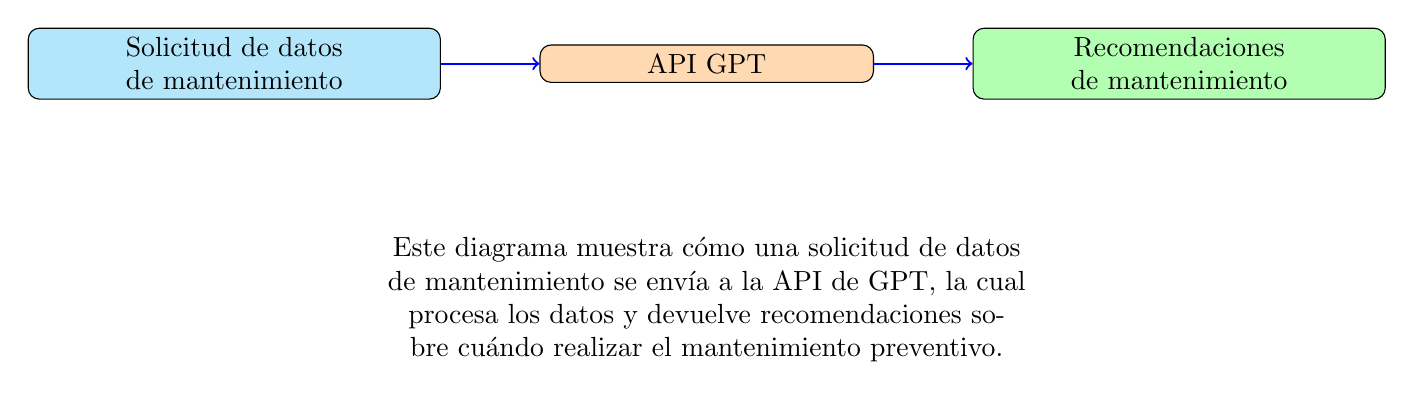
\begin{tikzpicture}[node distance=3cm]

    % Nodo para la solicitud de datos de mantenimiento
    \node (request) [draw, rectangle, fill=cyan!30, text width=5cm, align=center, rounded corners] 
    {Solicitud de datos de mantenimiento};

    % Nodo para la API de GPT
    \node (api) [right of=request, draw, rectangle, fill=orange!30, text width=4cm, align=center, rounded corners, xshift=3cm] 
    {API GPT};

    % Nodo para la respuesta generada
    \node (response) [right of=api, draw, rectangle, fill=green!30, text width=5cm, align=center, rounded corners, xshift=3cm] 
    {Recomendaciones de mantenimiento};

    % Conectar los nodos con flechas
    \draw[->, thick, blue] (request) -- (api);
    \draw[->, thick, blue] (api) -- (response);
    
    % Añadir un nodo de explicación
    \node (explanation) [below of=api, node distance=3cm, text width=10cm, align=center] 
    {Este diagrama muestra cómo una solicitud de datos de mantenimiento se envía a la API de GPT, 
    la cual procesa los datos y devuelve recomendaciones sobre cuándo realizar el mantenimiento preventivo.};

\end{tikzpicture}

\subsection{¿Dónde Encajan los Datos de mi Organización?}\label{donde-encajan-los-datos}

Uno de los primeros pasos para aprovechar la \textbf{inteligencia artificial (IA)} en una maquiladora es entender los tipos de datos que posee y cómo pueden utilizarse. Dependiendo de si los datos son estructurados o no estructurados, se pueden aplicar diferentes enfoques de IA, como \textbf{Machine Learning (ML)} o \textbf{Modelos de Lenguaje Extensos (LLMs)}.

\section{Modelos de Lenguaje Extensos (LLMs) como Primer Paso hacia el Uso de IA}\label{llms-primer-paso-ia}

Aunque los datos estructurados suelen encajar mejor con los algoritmos tradicionales de \textbf{Machine Learning (ML)}, los \textbf{Modelos de Lenguaje Extensos (LLMs)} pueden ser una excelente manera de comenzar a implementar inteligencia artificial en una maquiladora u otro entorno industrial.

Los LLMs, como \textbf{GPT-4} y \textbf{Gemini}, son herramientas poderosas que pueden interpretar grandes cantidades de texto no estructurado, como informes, correos electrónicos, y descripciones de problemas, lo que les permite ofrecer soluciones inmediatas o primeros pasos hacia la automatización.

\subsection{LLMs como Complemento al Machine Learning}
Si bien los algoritmos de ML tradicionales se enfocan en trabajar con datos numéricos estructurados (como métricas de producción, tiempos de ciclo o datos de sensores), los LLMs pueden ser útiles en el análisis de datos textuales no estructurados o en la generación de recomendaciones iniciales. Por ejemplo, en una maquiladora, los LLMs pueden analizar reportes de mantenimiento o de calidad para identificar patrones clave que, más adelante, podrían ser utilizados en modelos tradicionales de ML.

Además, los LLMs pueden interactuar con los datos de manera conversacional, lo que facilita su adopción en los primeros pasos de implementación de IA. Esto permite que los empleados, sin necesidad de conocimientos técnicos profundos, comiencen a beneficiarse de la IA a través de interfaces más accesibles.

\subsection{Comparación de Precisión: LLMs vs Algoritmos de Machine Learning}
Aunque los LLMs tienen capacidades impresionantes para manejar lenguaje natural, en el contexto de predicciones numéricas o análisis basados en datos estructurados, su precisión puede ser algo menor en comparación con los algoritmos tradicionales de \textbf{Machine Learning}. A continuación, se muestra una tabla que compara la precisión promedio de los LLMs frente a algoritmos tradicionales de ML.

\begin{table}[htbp]
\centering
\caption{Comparación de precisión entre Modelos de Lenguaje Extensos (LLMs) y algoritmos tradicionales de Machine Learning (ML) en tareas comunes.}
\label{tab:precision-llm-ml}
\begin{tabularx}{\textwidth}{|X|X|X|}
\hline
\textbf{Tipo de Algoritmo} & \textbf{Modelo/Algoritmo} & \textbf{Precisión Promedio (\%)} \\
\hline
\textbf{Modelos de Lenguaje Extensos (LLMs)} & GPT-4, Gemini, otros modelos generativos & 65-73\% en predicciones numéricas o tareas de análisis de datos estructurados \\
\hline
\textbf{Algoritmos Tradicionales de Machine Learning} & Regresión Lineal, Redes Neuronales, Bosques Aleatorios, SVM & 85-95\% en predicciones numéricas y análisis de datos estructurados \\
\hline
\end{tabularx}
\end{table}

\subsection{Ventajas de Usar LLMs en el Primer Paso hacia la IA}
Los LLMs pueden ser una excelente opción para comenzar a integrar IA en una organización debido a las siguientes ventajas:
\begin{itemize}
    \item \textbf{Accesibilidad:} Los LLMs permiten a los usuarios interactuar con la IA mediante lenguaje natural, lo que reduce la barrera de entrada para su uso.
    \item \textbf{Flexibilidad:} Pueden manejar una amplia variedad de datos textuales no estructurados, como reportes, correos electrónicos y descripciones técnicas.
    \item \textbf{Rapidez en implementación:} Es más rápido implementar LLMs para análisis iniciales, lo que permite obtener valor de los datos sin tener que estructurarlos completamente desde el principio.
\end{itemize}

\subsection{Limitaciones de los LLMs en comparación con Machine Learning}
A pesar de sus ventajas, los LLMs presentan algunas limitaciones cuando se comparan con los algoritmos tradicionales de ML:
\begin{itemize}
    \item \textbf{Menor precisión en tareas numéricas:} Como se muestra en la Tabla \ref{tab:precision-llm-ml}, los LLMs tienen una precisión menor al analizar datos estructurados o numéricos.
    \item \textbf{No son ideales para predicciones complejas basadas en datos históricos:} Los algoritmos de ML, como las redes neuronales y los bosques aleatorios, siguen siendo más adecuados para análisis predictivos complejos.
    \item \textbf{Requieren mayor capacidad computacional:} Aunque los LLMs son poderosos, su costo computacional es generalmente mayor que el de los modelos tradicionales de ML.
\end{itemize}

\subsection{Conclusión: LLMs como Puerta de Entrada a la IA}
En resumen, los LLMs pueden ser una herramienta poderosa para que las organizaciones comiencen su viaje hacia la automatización inteligente. Aunque no alcanzan la misma precisión que los algoritmos tradicionales de Machine Learning en ciertos tipos de tareas, su capacidad para interactuar con datos no estructurados y su accesibilidad los convierten en una opción ideal para dar los primeros pasos en la implementación de IA.

``Los LLMs son la puerta de entrada hacia el mundo del Machine Learning, proporcionando un puente accesible entre la interacción humana y la automatización avanzada.''

\section{¿Dónde Encajan los Datos de mi Organización?}\label{donde-encajan-los-datos}

Uno de los primeros pasos para aprovechar la \textbf{inteligencia artificial (IA)} en una maquiladora es entender los tipos de datos que posee y cómo pueden utilizarse. Dependiendo de si los datos son estructurados o no estructurados, se pueden aplicar diferentes enfoques de IA, como \textbf{Machine Learning (ML)} o \textbf{Modelos de Lenguaje Extensos (LLMs)}.

\begin{table}[htbp]
\centering
\caption{Ejemplos de tipos de datos en una maquiladora y aplicaciones de Machine Learning (ML) y Modelos de Lenguaje Extensos (LLMs).}
\begin{tabularx}{\textwidth}{|X|X|X|X|}
\hline
\textbf{Tipo de Datos} & \textbf{Descripción} & \textbf{Modelo Adecuado} & \textbf{Ejemplo de Aplicación} \\
\hline
Numéricos estructurados & Datos organizados en tablas o bases de datos, como registros de producción diaria, tiempos de ciclo, consumo de energía. & Machine Learning (ML) & Predicción de fallos de máquinas, optimización de inventario, análisis de tiempos de ciclo. \\
\hline
Texto no estructurado & Informes de mantenimiento, correos electrónicos, descripciones de problemas técnicos. & Modelos de Lenguaje Extensos (LLM) & Análisis de reportes de fallos, generación automática de resúmenes, asistente virtual para consultas sobre mantenimiento. \\
\hline
Imágenes & Fotografías capturadas por cámaras de control de calidad en las líneas de producción para detectar defectos. & Machine Learning (ML) & Detección de defectos mediante visión por computadora, inspección de calidad automatizada. \\
\hline
Datos de sensores (IoT) & Sensores conectados a máquinas, como temperatura, vibración, velocidad de operación. & Machine Learning (ML) & Mantenimiento predictivo, monitoreo en tiempo real, optimización de eficiencia energética. \\
\hline
Datos de PLC (Programmable Logic Controller) & Datos generados por controladores lógicos programables, como ciclos de máquina y activación de actuadores. & Machine Learning (ML) & Optimización de la programación del PLC, detección de patrones anormales, mantenimiento predictivo. \\
\hline
Datos SMT (Surface-Mount Technology) & Registros de colocación de componentes, tiempos de ciclo, análisis de defectos de ensamblaje en productos electrónicos. & Machine Learning (ML) & Optimización de líneas SMT, reducción de scrap, análisis de defectos en fabricación electrónica. \\
\hline
Datos médicos ocupacionales & Información sobre la salud de los trabajadores, como ritmo cardíaco y niveles de estrés en tiempo real. & Machine Learning (ML) & Prevención de riesgos laborales, monitoreo de salud en tiempo real, optimización de turnos según fatiga. \\
\hline
Datos de seguridad laboral & Registros de accidentes laborales, incumplimientos de normas, condiciones ambientales peligrosas. & Machine Learning (ML) & Prevención de accidentes mediante análisis predictivo, alertas automáticas de condiciones peligrosas. \\
\hline
Datos de control de calidad & Métricas de calidad y pruebas de resistencia o durabilidad, tanto destructivas como no destructivas. & Machine Learning (ML) & Análisis predictivo de calidad, optimización de procesos de inspección, ajuste de parámetros en tiempo real. \\
\hline
Datos energéticos & Medición de consumo de energía por máquinas y líneas de producción. & Machine Learning (ML) & Optimización del consumo energético, predicción de picos de consumo, reducción de costos energéticos. \\
\hline
\end{tabularx}
\label{tab:responsive-table}
\end{table}

\section{Modelos de Lenguaje Extensos (LLMs) como Primer Paso hacia el Uso de IA}\label{llms-primer-paso-ia}

Aunque los datos estructurados suelen encajar mejor con los algoritmos tradicionales de \textbf{Machine Learning (ML)}, los \textbf{Modelos de Lenguaje Extensos (LLMs)} pueden ser una excelente manera de comenzar a implementar inteligencia artificial en una maquiladora u otro entorno industrial.

Los LLMs, como \textbf{GPT-4} y \textbf{Gemini}, son herramientas poderosas que pueden interpretar grandes cantidades de texto no estructurado, como informes, correos electrónicos, y descripciones de problemas, lo que les permite ofrecer soluciones inmediatas o primeros pasos hacia la automatización.

\subsection{LLMs como Complemento al Machine Learning}
Si bien los algoritmos de ML tradicionales se enfocan en trabajar con datos numéricos estructurados (como métricas de producción, tiempos de ciclo o datos de sensores), los LLMs pueden ser útiles en el análisis de datos textuales no estructurados o en la generación de recomendaciones iniciales. Por ejemplo, en una maquiladora, los LLMs pueden analizar reportes de mantenimiento o de calidad para identificar patrones clave que, más adelante, podrían ser utilizados en modelos tradicionales de ML.

Además, los LLMs pueden interactuar con los datos de manera conversacional, lo que facilita su adopción en los primeros pasos de implementación de IA. Esto permite que los empleados, sin necesidad de conocimientos técnicos profundos, comiencen a beneficiarse de la IA a través de interfaces más accesibles.

\subsection{Comparación de Precisión: LLMs vs Algoritmos de Machine Learning}
Aunque los LLMs tienen capacidades impresionantes para manejar lenguaje natural, en el contexto de predicciones numéricas o análisis basados en datos estructurados, su precisión puede ser algo menor en comparación con los algoritmos tradicionales de \textbf{Machine Learning}. A continuación, se muestra una tabla que compara la precisión promedio de los LLMs frente a algoritmos tradicionales de ML.

\begin{table}[htbp]
\centering
\caption{Comparación de precisión entre Modelos de Lenguaje Extensos (LLMs) y algoritmos tradicionales de Machine Learning (ML) en tareas comunes.}
\label{tab:precision-llm-ml}
\begin{tabularx}{\textwidth}{|X|X|X|}
\hline
\textbf{Tipo de Algoritmo} & \textbf{Modelo/Algoritmo} & \textbf{Precisión Promedio (\%)} \\
\hline
\textbf{Modelos de Lenguaje Extensos (LLMs)} & GPT-4, Gemini, otros modelos generativos & 65-73\% en predicciones numéricas o tareas de análisis de datos estructurados \\
\hline
\textbf{Algoritmos Tradicionales de Machine Learning} & Regresión Lineal, Redes Neuronales, Bosques Aleatorios, SVM & 85-95\% en predicciones numéricas y análisis de datos estructurados \\
\hline
\end{tabularx}
\end{table}

\subsection{Ventajas de Usar LLMs en el Primer Paso hacia la IA}
Los LLMs pueden ser una excelente opción para comenzar a integrar IA en una organización debido a las siguientes ventajas:
\begin{itemize}
    \item \textbf{Accesibilidad:} Los LLMs permiten a los usuarios interactuar con la IA mediante lenguaje natural, lo que reduce la barrera de entrada para su uso.
    \item \textbf{Flexibilidad:} Pueden manejar una amplia variedad de datos textuales no estructurados, como reportes, correos electrónicos y descripciones técnicas.
    \item \textbf{Rapidez en implementación:} Es más rápido implementar LLMs para análisis iniciales, lo que permite obtener valor de los datos sin tener que estructurarlos completamente desde el principio.
\end{itemize}

\subsection{Limitaciones de los LLMs en comparación con Machine Learning}
A pesar de sus ventajas, los LLMs presentan algunas limitaciones cuando se comparan con los algoritmos tradicionales de ML:
\begin{itemize}
    \item \textbf{Menor precisión en tareas numéricas:} Como se muestra en la Tabla \ref{tab:precision-llm-ml}, los LLMs tienen una precisión menor al analizar datos estructurados o numéricos.
    \item \textbf{No son ideales para predicciones complejas basadas en datos históricos:} Los algoritmos de ML, como las redes neuronales y los bosques aleatorios, siguen siendo más adecuados para análisis predictivos complejos.
    \item \textbf{Requieren mayor capacidad computacional:} Aunque los LLMs son poderosos, su costo computacional es generalmente mayor que el de los modelos tradicionales de ML.
\end{itemize}

\subsection{Conclusión: LLMs como Puerta de Entrada a la IA}
En resumen, los LLMs pueden ser una herramienta poderosa para que las organizaciones comiencen su viaje hacia la automatización inteligente. Aunque no alcanzan la misma precisión que los algoritmos tradicionales de Machine Learning en ciertos tipos de tareas, su capacidad para interactuar con datos no estructurados y su accesibilidad los convierten en una opción ideal para dar los primeros pasos en la implementación de IA.

``Los LLMs son la puerta de entrada hacia el mundo del Machine Learning, proporcionando un puente accesible entre la interacción humana y la automatización avanzada.''
